%%=============================================================================
%% Voorbereiding op onderzoek
%%=============================================================================

\chapter{Voorbereiding op onderzoek}
\label{ch:Voorbereiding op onderzoek}

\section{Opnemen trainingsdata}
\label{sec:Opnemen trainingsdata}

Zoals eerder aangehaald in dit werkstuk dienen de frameworks getraind te worden met een aantal afbeeldingen om voorspellingen te doen. De foto’s zijn genomen een iPhone 8, die een 12-MP camera bevat. Er zijn telkens dertig opnames gemaakt van elk product. De helft daarvan zijn met een witte achtergrond, de andere helft met een zwarte achtergrond telkens met een resolutie van 3024 x 4032 of 4032 x 3024 daarna werden de afbeeldingen verkleind tot een grootte van respectievelijk 300 x 400 of 400 x 300. Zo kunnen de afbeeldingen makkelijker verwerkt worden door de frameworks. Per foto, per achtergrond is er steeds rond het product gegaan met de camera. Zo leert het framework het product herkennen uit verschillende hoeken. Om het onderzoek zo nauwkeurig mogelijk te houden zijn de trainingsafbeeldingen per product nagenoeg hetzelfde. 

Per categorie producten zijn er iedere keer drie producten gekozen die minimaal verschillen ten opzichte van elkaar. Zo is er een duidelijk beeld hoe goed een framework de details controleert. Dit is een vereiste wil men een framework toepassen in de praktijk voor productherkenning aangezien behoorlijk wat producten bijna dezelfde verpakking hebben.

\subsection{Kleine producten}
\label{ssec:Kleine producten}

Voor de kleine producten zijn er drie verschillende wimpers gekozen die waarvan de doos sterkt lijk op de andere. De eerste twee artikels verschillen van kleur, de derde wimper heeft verscheidene kleuren maar bevat ook de kleuren van de eerste twee wimpers.
Figuren \ref{fig:pinkFeathers}, \ref{fig:80neonGreen} en \ref{fig:neonFeathers} tonen de gebruikte trainingsdata per product.

\begin{figure}[!ht]
    \centering
        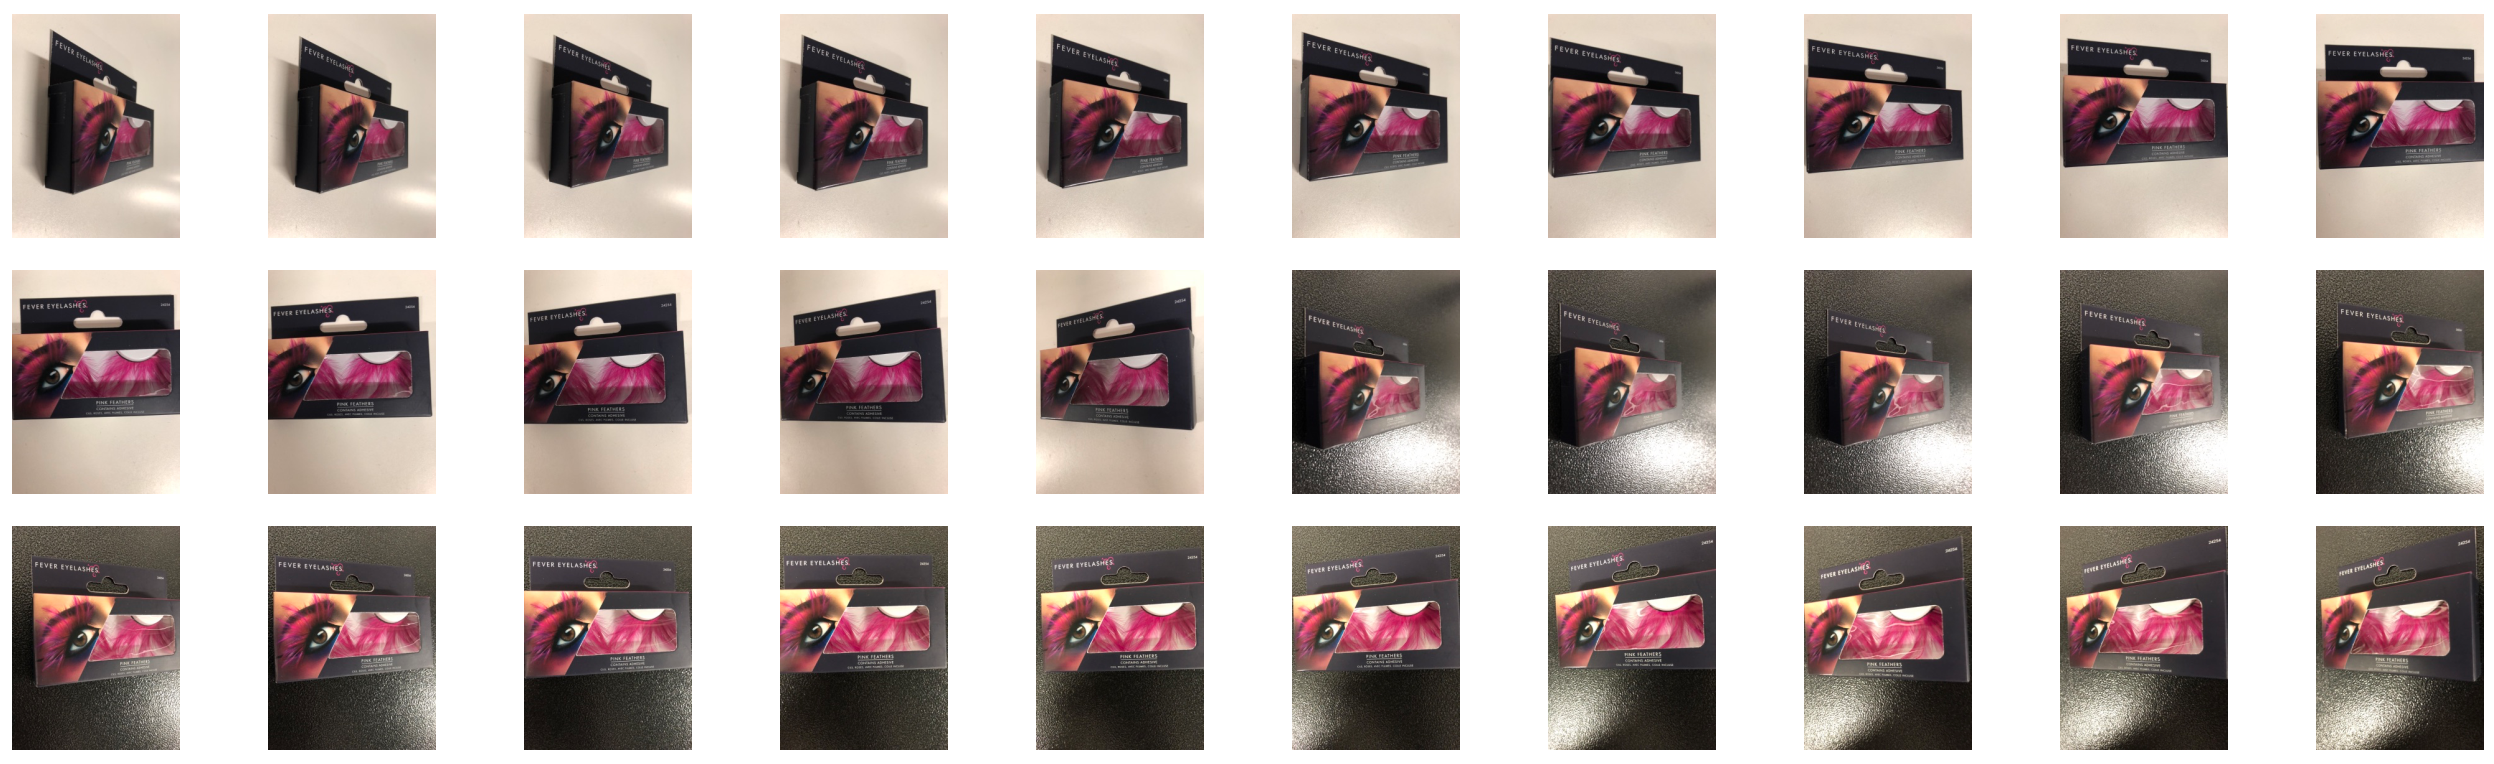
\includegraphics[width=1\textwidth]{img/pinkFeathers.png}
    \caption{Trainingsdata voor het product 'pinkFeathers'}
    \label{fig:pinkFeathers}
  \end{figure}

  \begin{figure}[!ht]
    \centering
        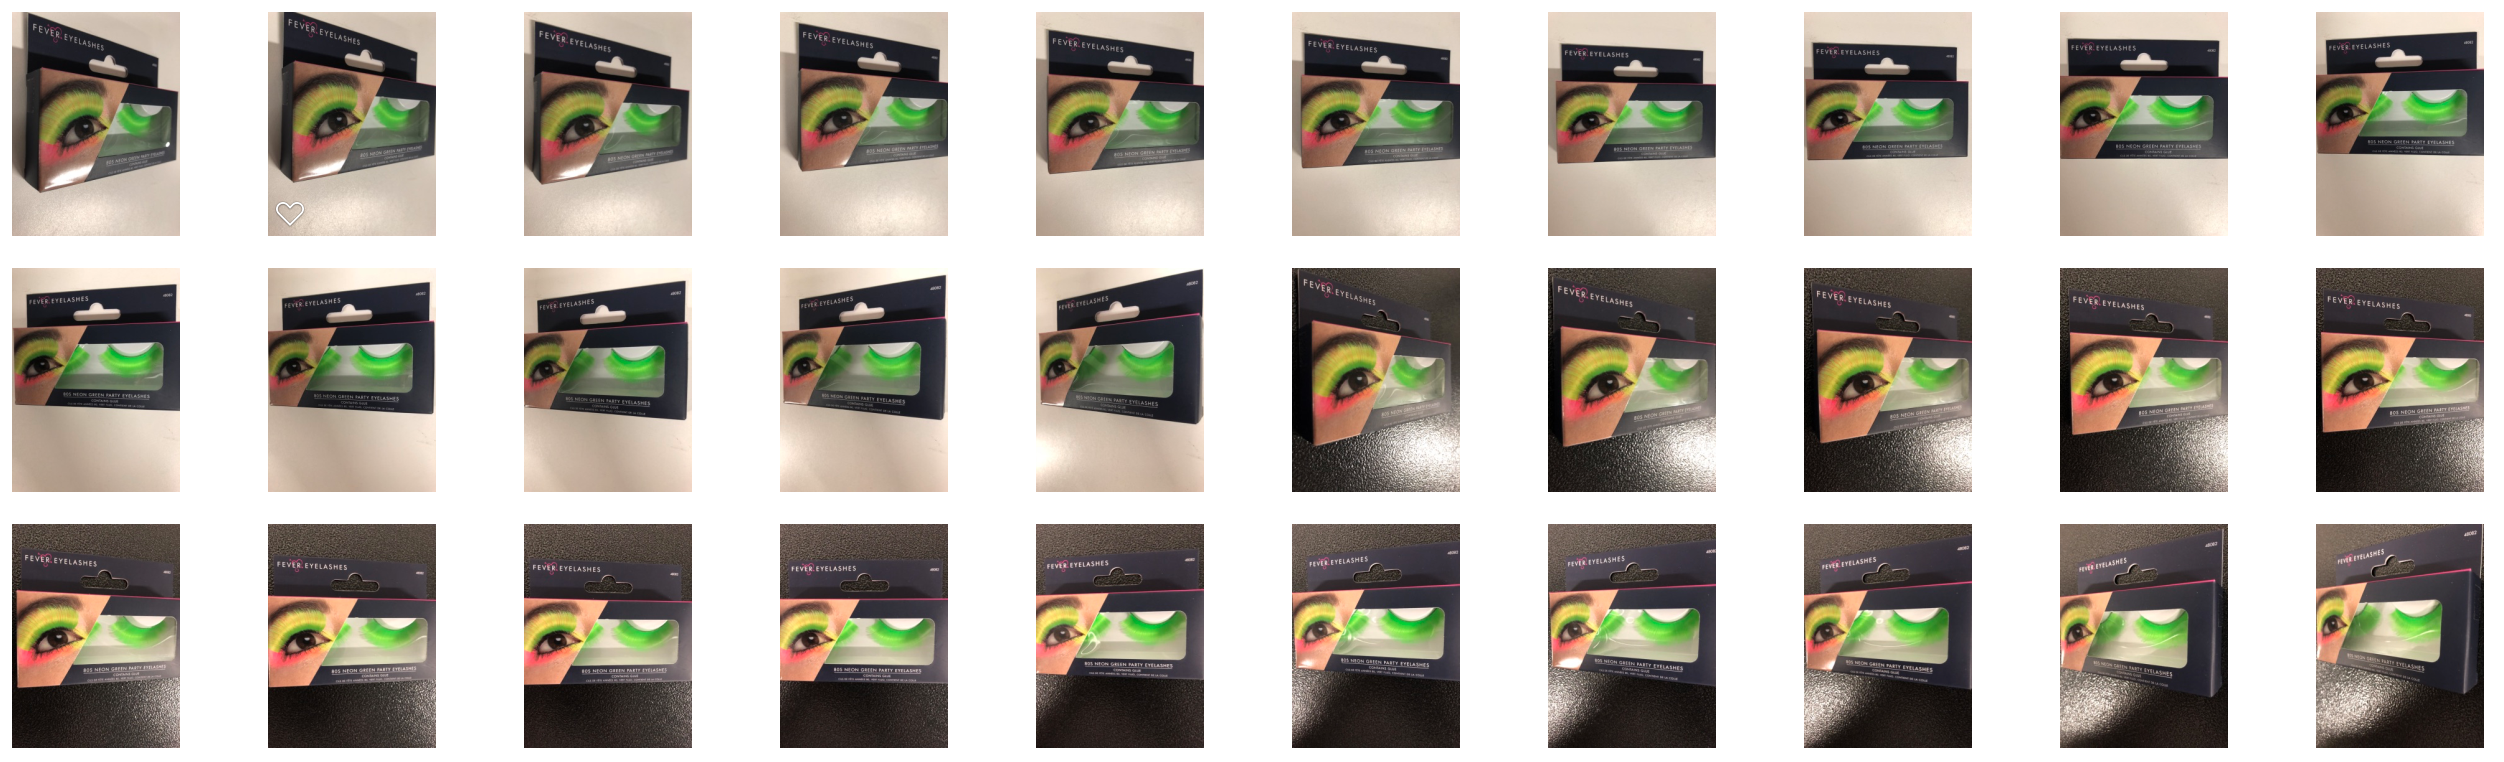
\includegraphics[width=1\textwidth]{img/80neonGreen.png}
    \caption{Trainingsdata voor het product '80neonGreen'}
    \label{fig:80neonGreen}
  \end{figure}

  \begin{figure}[h!]
    \centering
        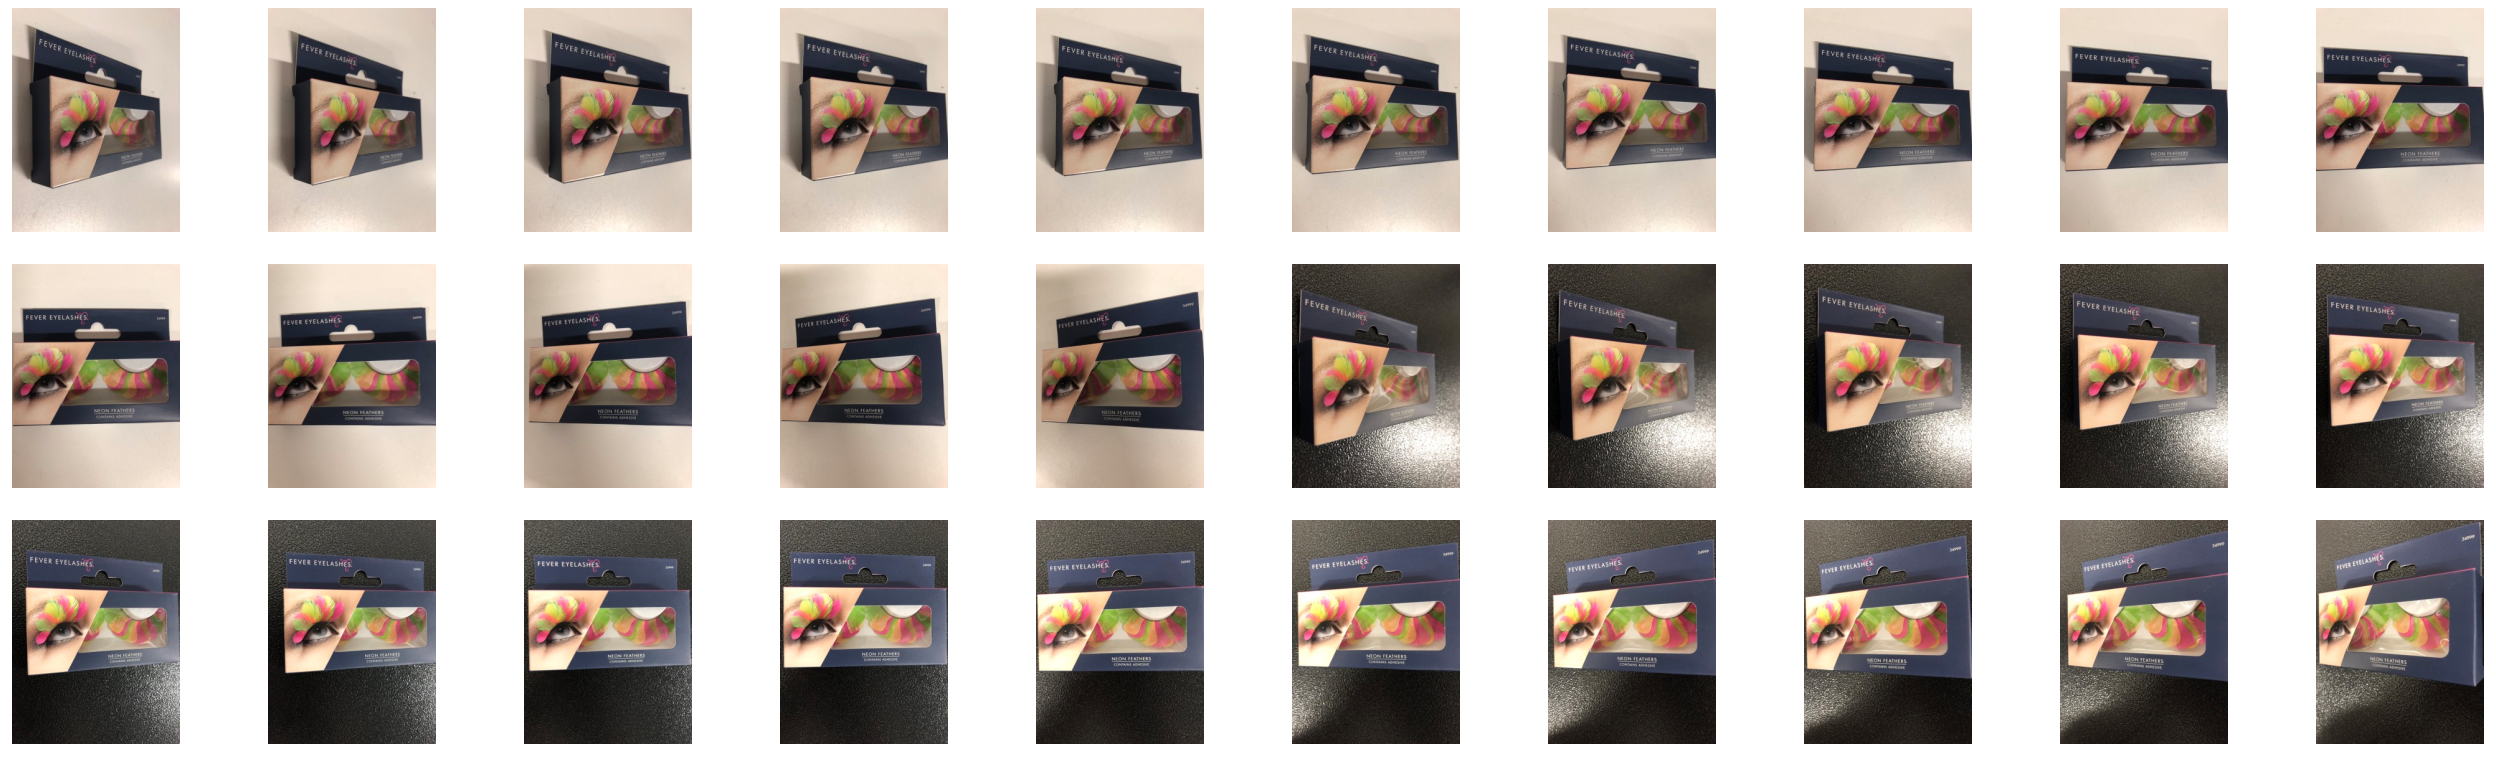
\includegraphics[width=1\textwidth]{img/neonFeathers.png}
    \caption{Trainingsdata voor het product 'neonFeathers'}
    \label{fig:neonFeathers}
  \end{figure}

  \subsection{Middelgrote producten}
\label{ssec:Middelgrote producten}

Voor deze artikels zijn afwijkend pruiken geselecteerd. Die hebben wel ongeveer dezelfde kleur, maar de vorm is verschillend. Op de verpakking staat een voorbeeld van de pruik. Buiten het voorbeeld zijn de dozen overeenkomstig met elkaar. 
Figuren \ref{fig:khloe}, \ref{fig:amber} en \ref{fig:sienna} geven de toegepaste trainingsdata weer per artikel.

\begin{figure}[h!]
    \centering
        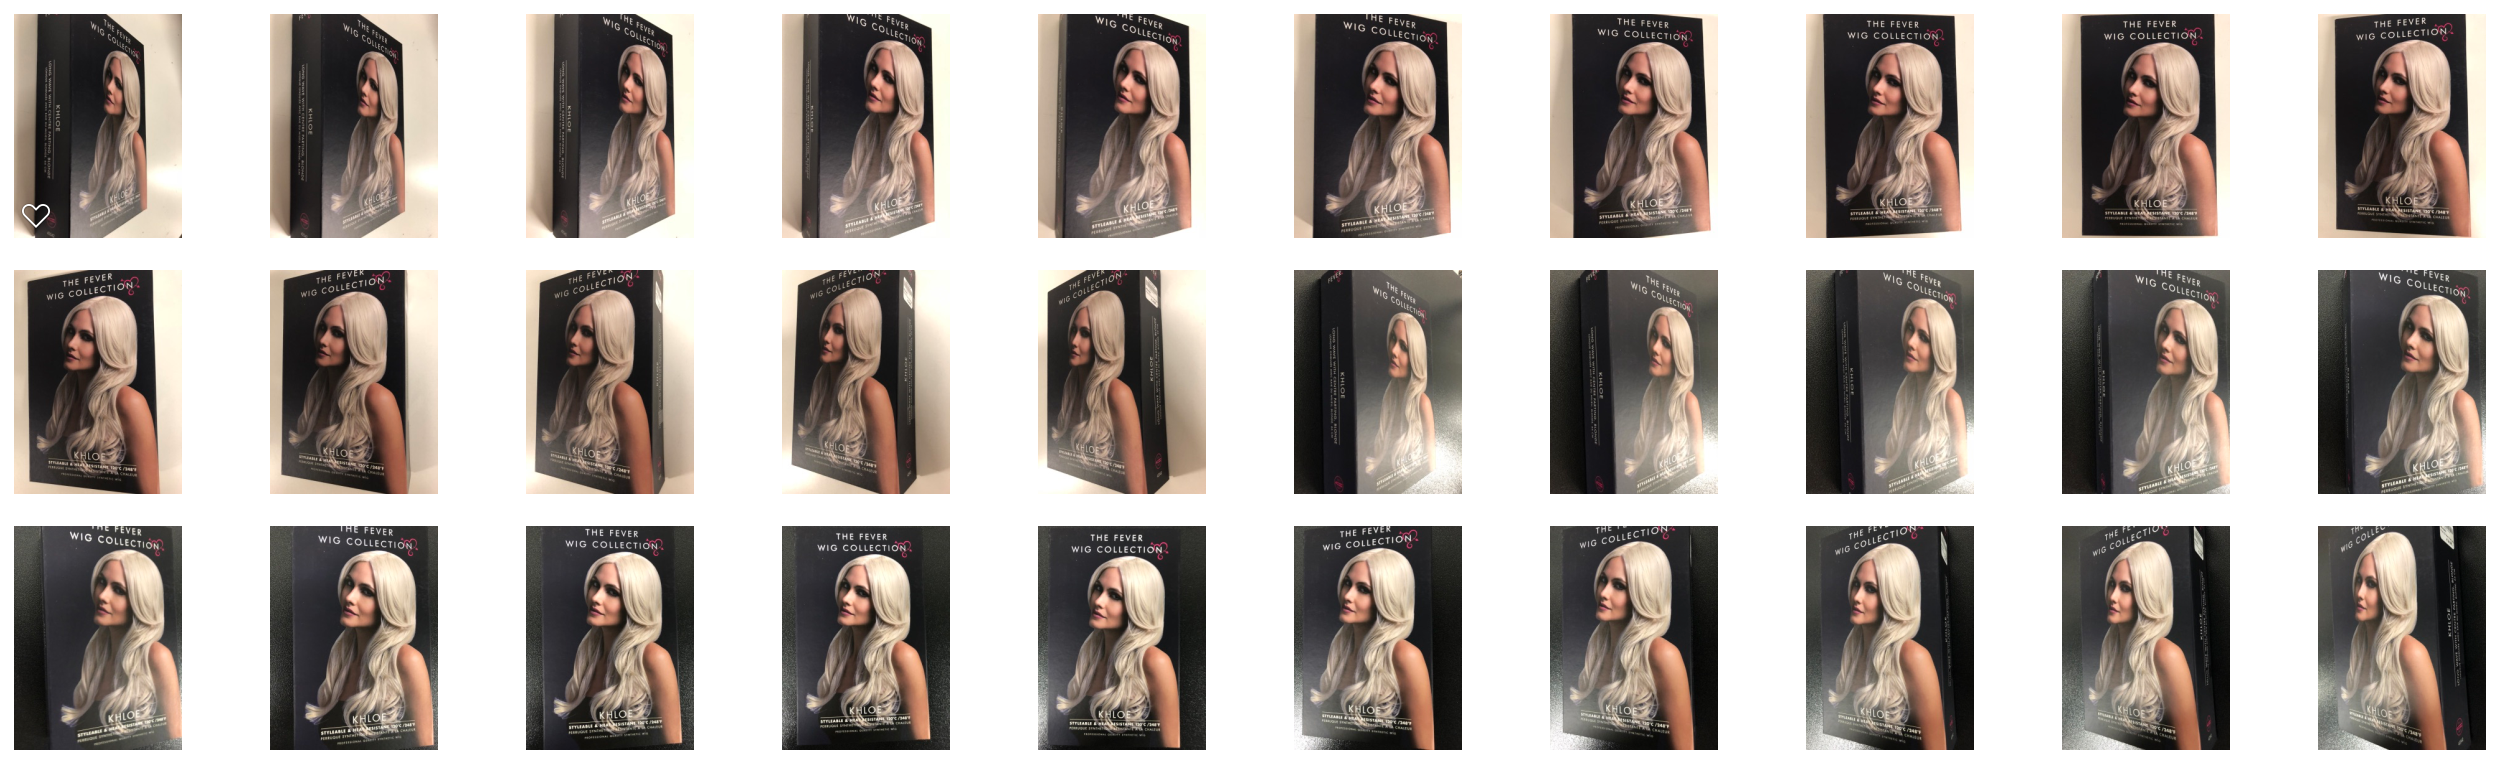
\includegraphics[width=1\textwidth]{img/khloe.png}
    \caption{Trainingsdata voor het product 'khloe'}
    \label{fig:khloe}
  \end{figure}

  \begin{figure}[h!]
    \centering
        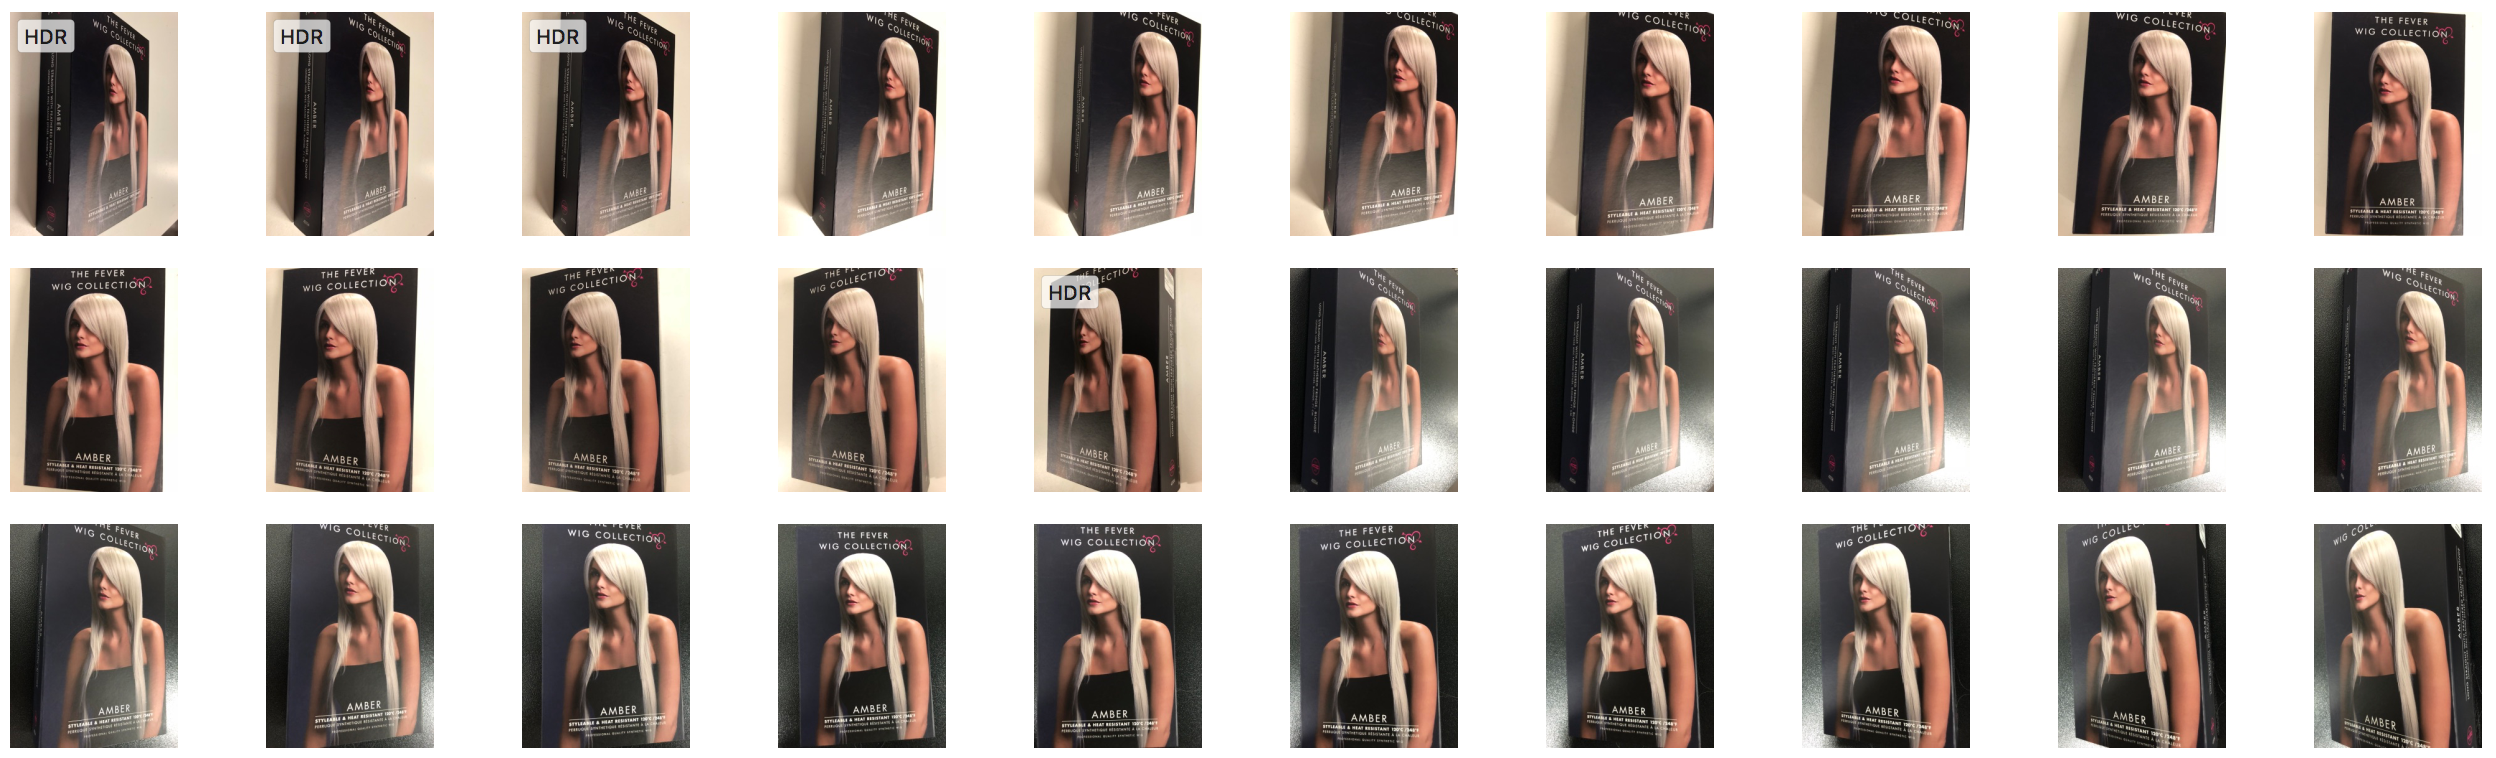
\includegraphics[width=1\textwidth]{img/amber.png}
    \caption{Trainingsdata voor het product 'amber'}
    \label{fig:amber}
  \end{figure}

  \begin{figure}[h!]
    \centering
        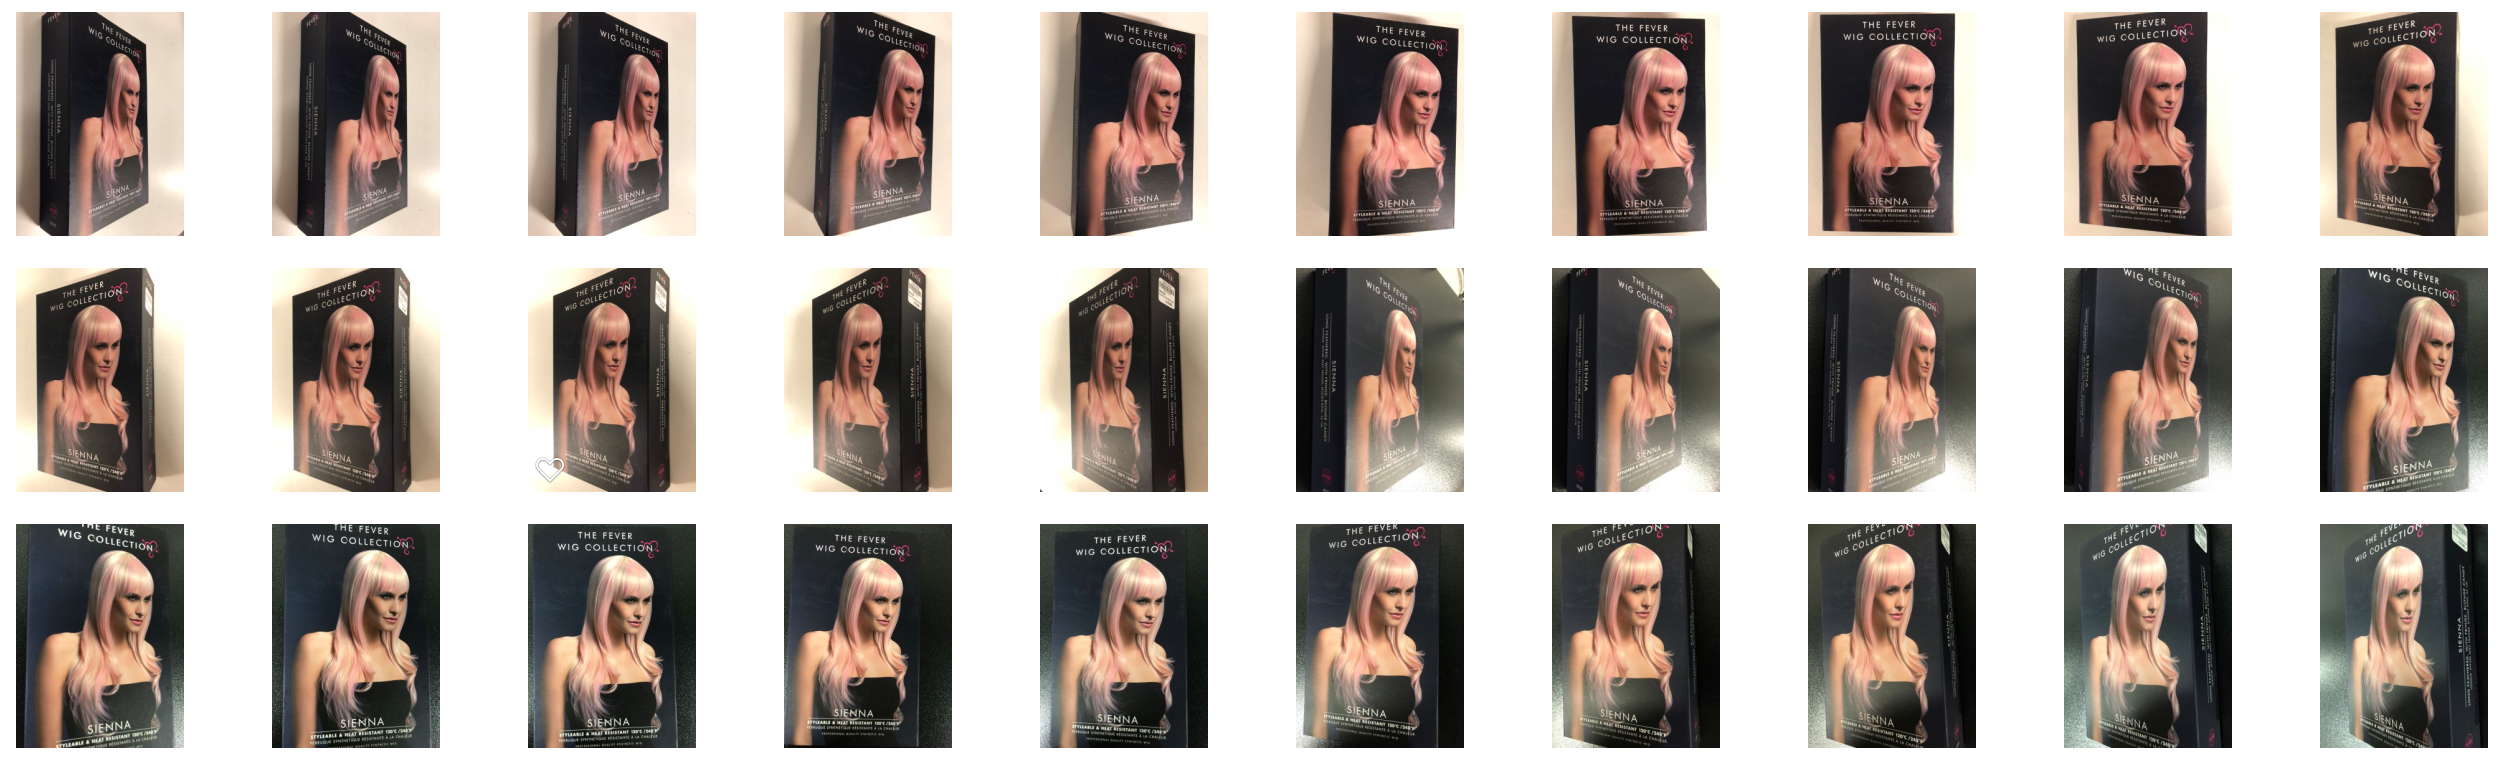
\includegraphics[width=1\textwidth]{img/sienna.png}
    \caption{Trainingsdata voor het product 'sienna'}
    \label{fig:sienna}
  \end{figure}

  \subsection{Grote producten}
  \label{ssec:Grote producten}

  Om deze groep producten te vullen met trainingsdata is gekozen voor drie verscheidene kostuums van de sprookjesfiguur ‘Alice’ van het alom bekend sprookje ‘Alice in wonderland’. Net zoals voorgaande groepen is de bijna identiek, behalve de illustratie van het kostuum. 
  Figuren \ref{fig:rebelAlice}, \ref{fig:delightfulAlice} en \ref{fig:hypnoticAlice} laten de afbeeldingen die gebruikt zijn als training zien.
  
  \begin{figure}[h!]
    \centering
        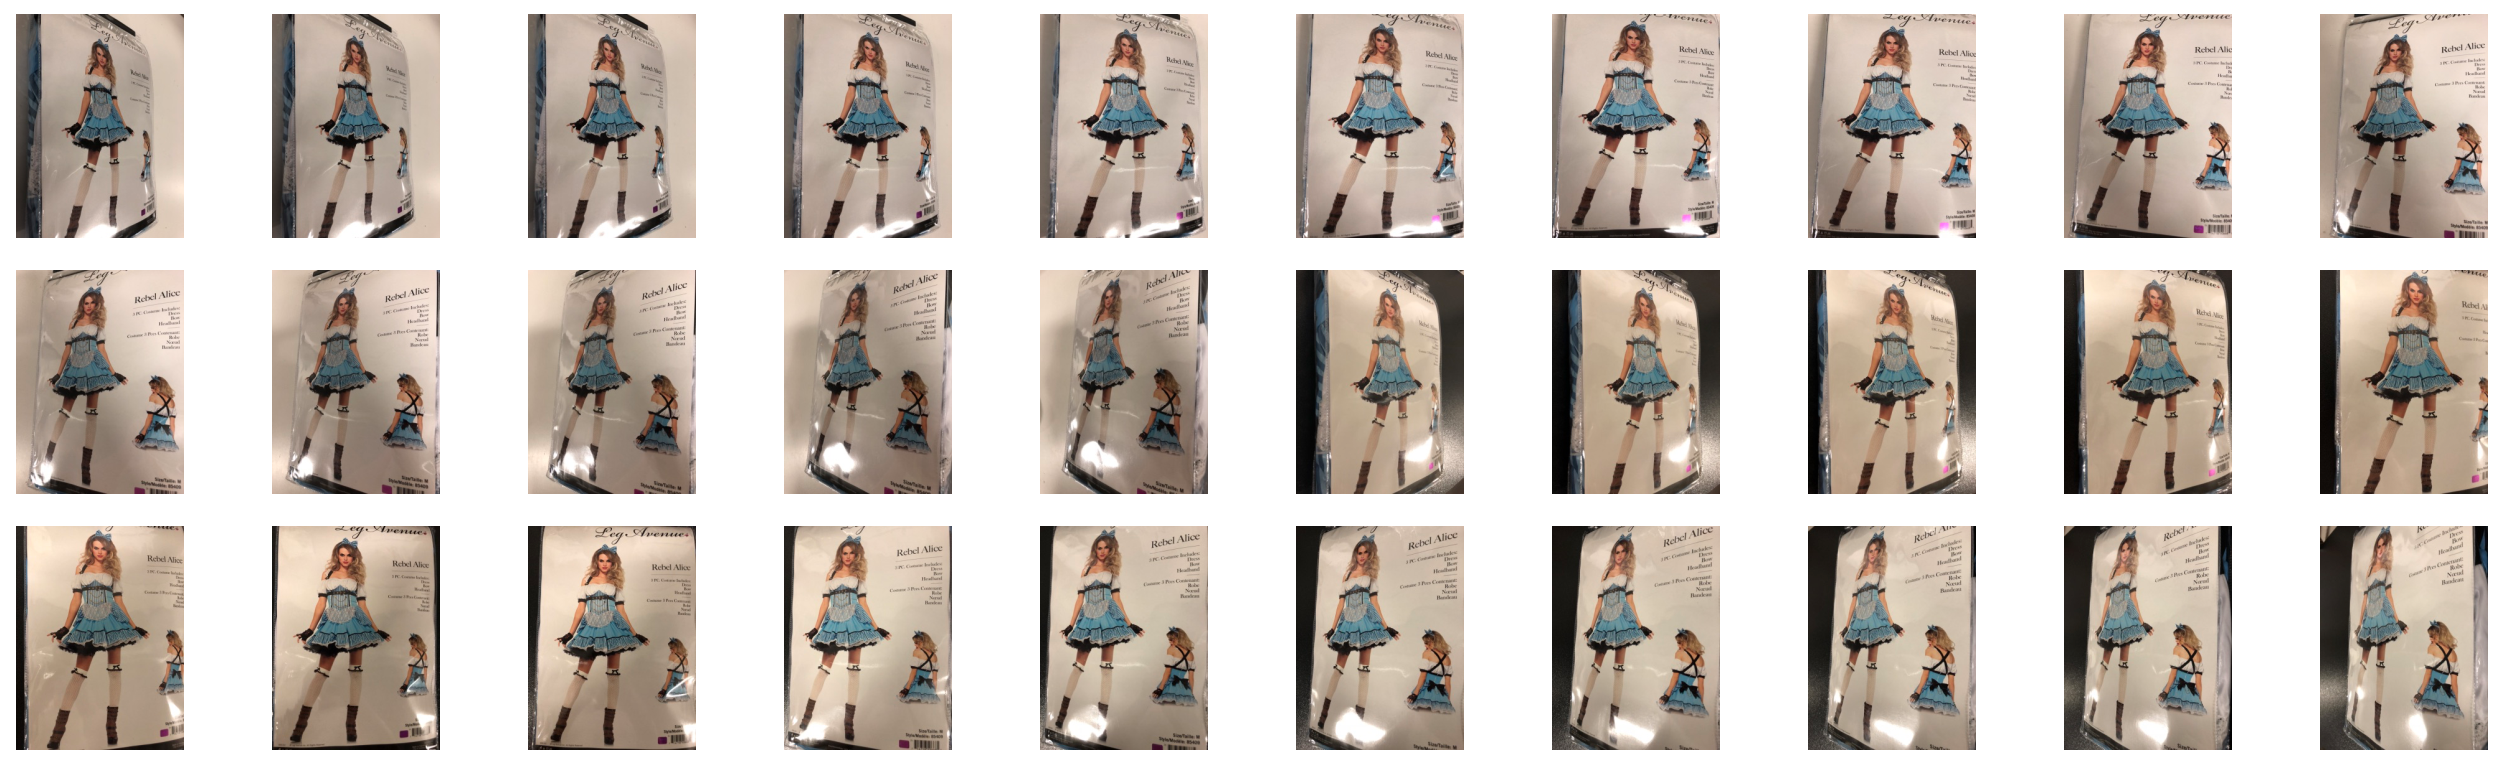
\includegraphics[width=1\textwidth]{img/rebelAlice.png}
    \caption{Trainingsdata voor het product 'rebelAlice'}
    \label{fig:rebelAlice}
  \end{figure}

  \begin{figure}[h!]
    \centering
        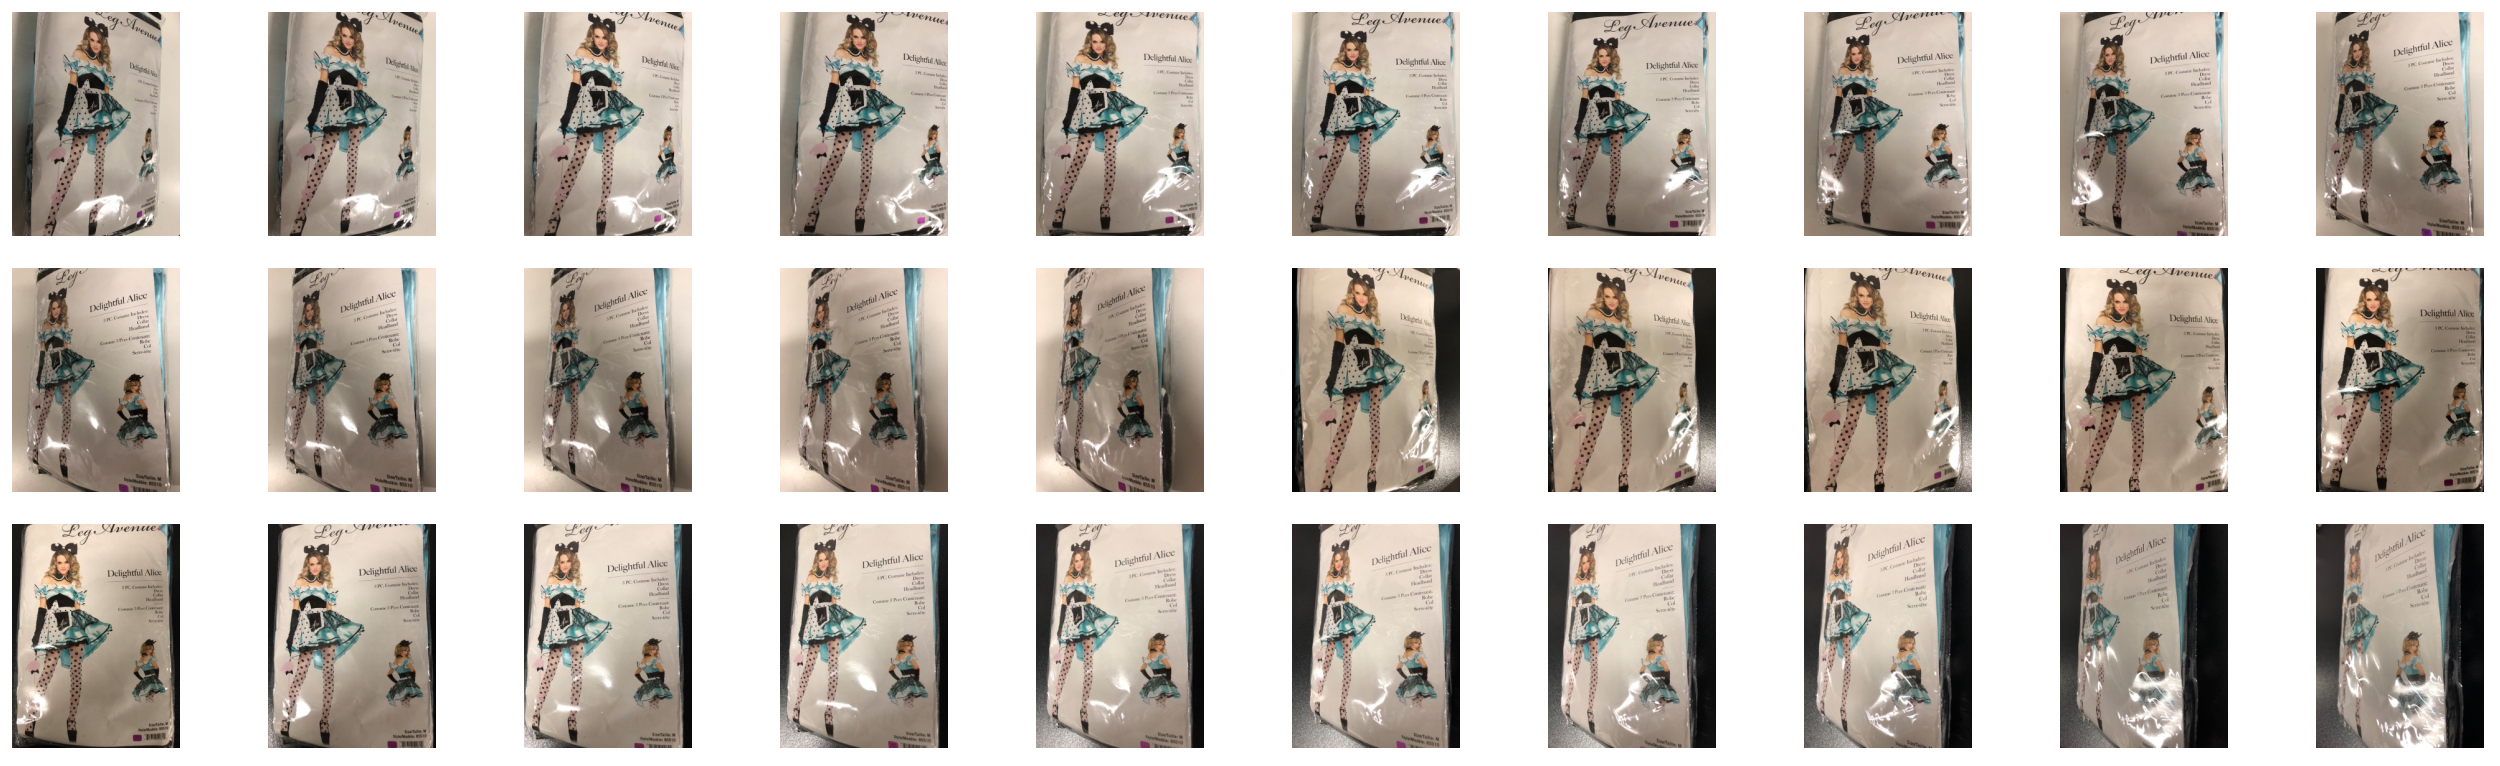
\includegraphics[width=1\textwidth]{img/delightfulAlice.png}
    \caption{Trainingsdata voor het product 'delightfulAlice'}
    \label{fig:delightfulAlice}
  \end{figure}

  \begin{figure}[h!]
    \centering
        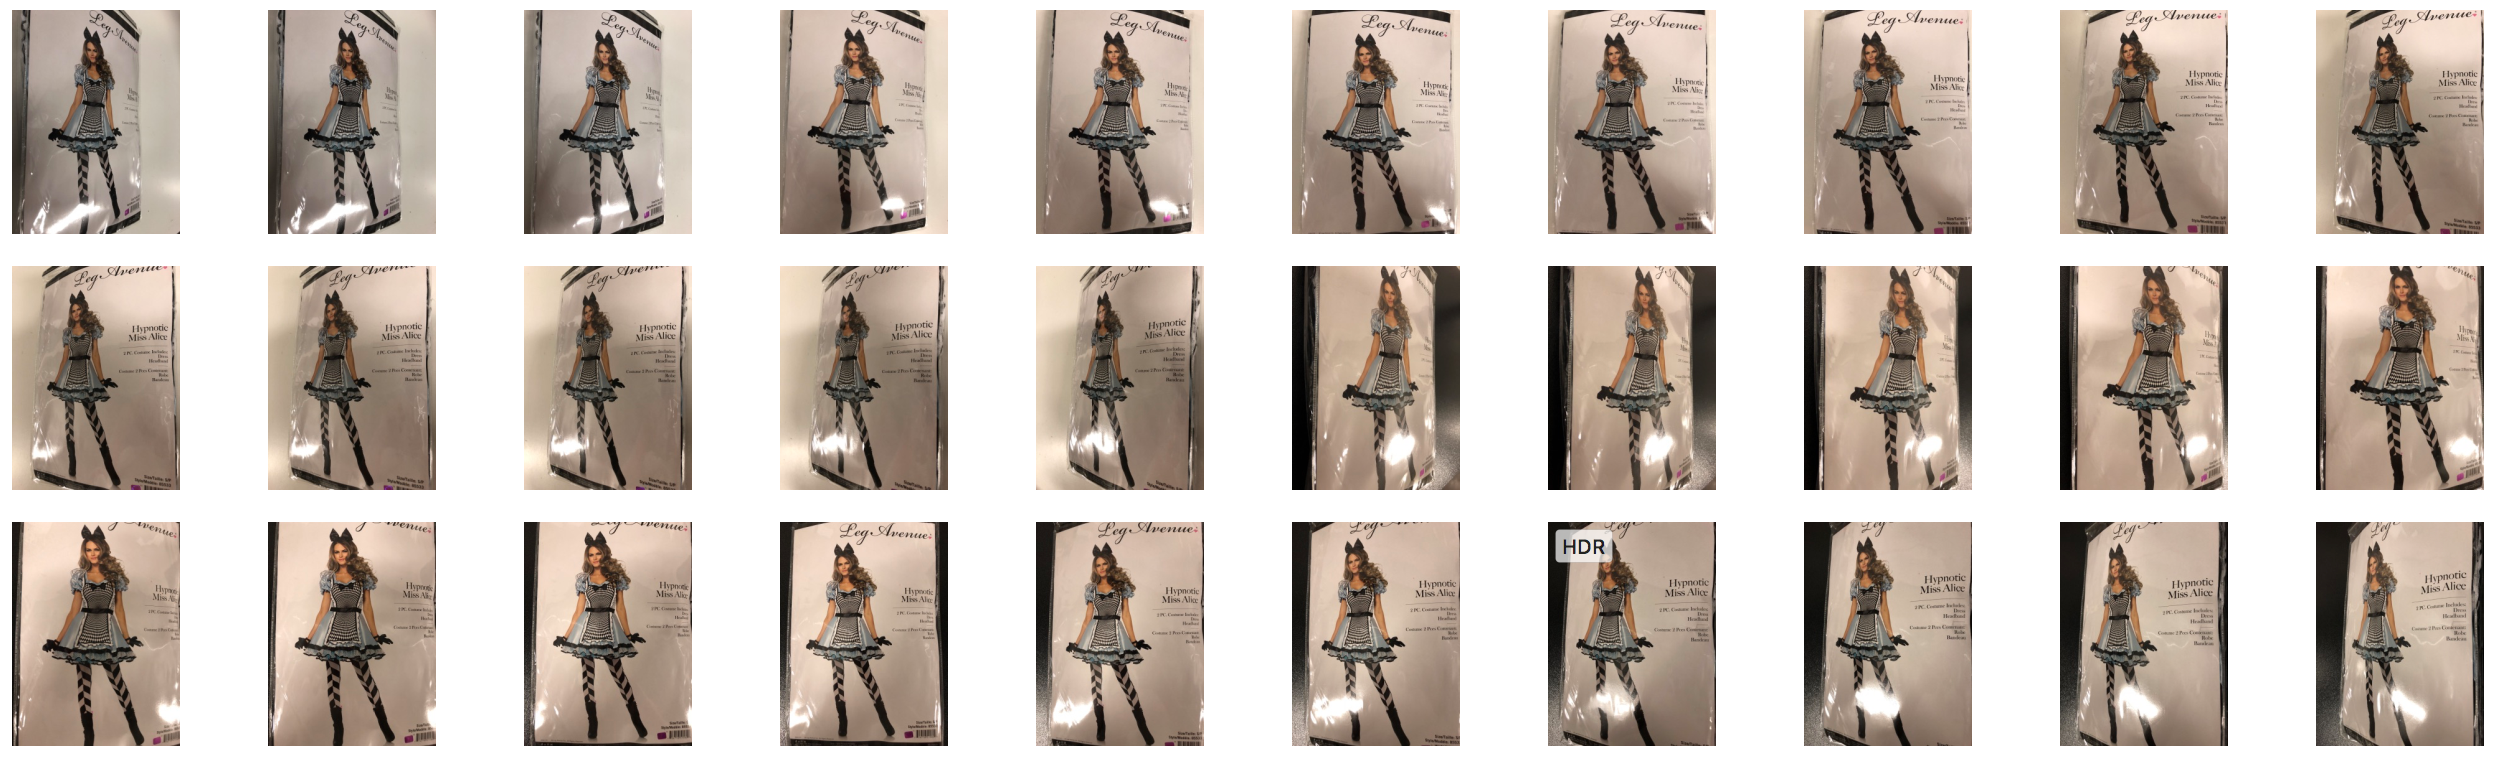
\includegraphics[width=1\textwidth]{img/hypnoticAlice.png}
    \caption{Trainingsdata voor het product 'hypnoticAlice'}
    \label{fig:hypnoticAlice}
  \end{figure}

  \section{Opnemen testdata}
  \label{sec:Opnemen testdata}

  Om de frameworks te toetsen op nauwkeurigheid zijn er per groep producten testfoto’s genomen. Per groep zitten drie gelijkaardige artikels, voor elk daarvan zijn er 10 testafbeeldingen. De testdata geeft een indicatie hoe de producten in realiteit zouden gescand worden. Vaak zal een persoon het product in de hand nemen en scannen, ofwel zal het product gescand worden vanuit het rek. Bij de data is ook rekening gehouden met verschillende afstanden tussen de smartphone en het product. Voor het opnemen van de testdata is net zoals voor het opnemen van de trainingsdata een iPhone 8 gebruikt.
  Figuren \ref{fig:testklein}, \ref{fig:testmiddel} en \ref{fig:testgroot} tonen de gebruikte testdata voor respectievelijk kleine, middelgrote en grote producten. 

  \begin{figure}[h!]
    \centering
        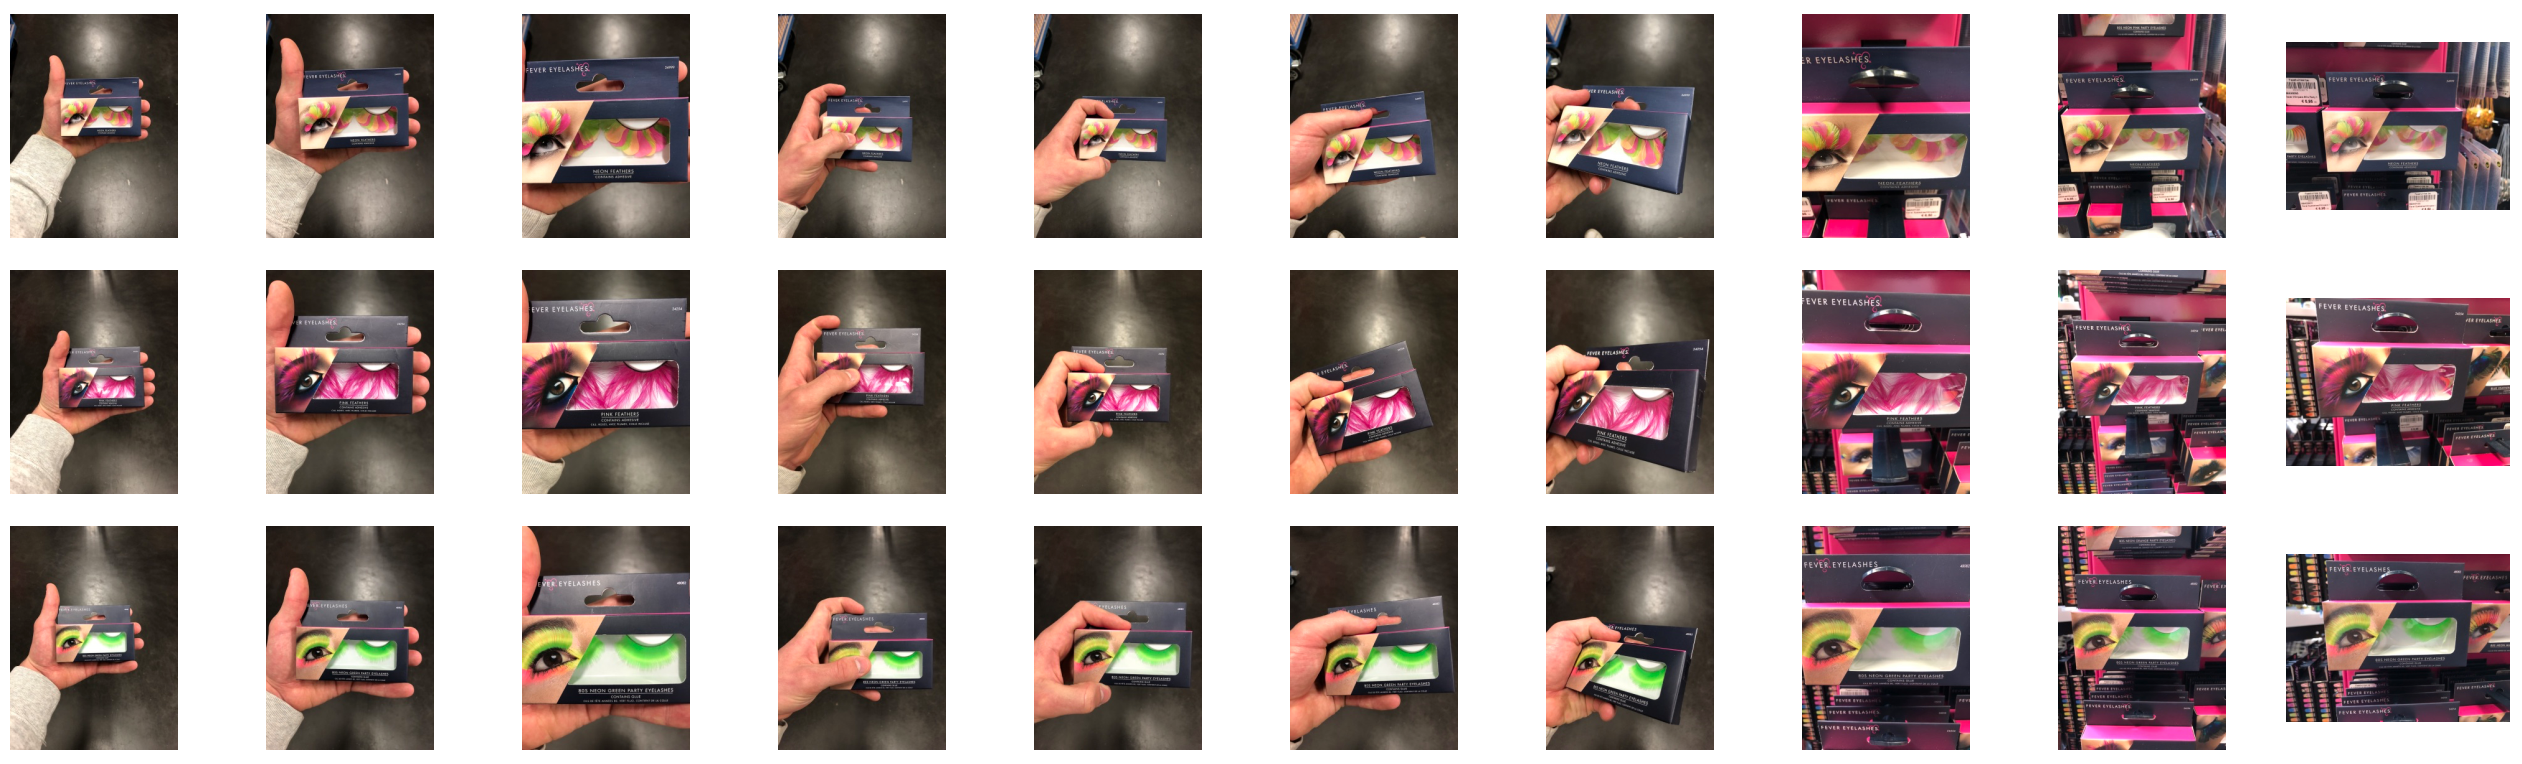
\includegraphics[width=1\textwidth]{img/testklein.png}
    \caption{Testdata voor kleine producten}
    \label{fig:testklein}
  \end{figure}

  \begin{figure}[h!]
    \centering
        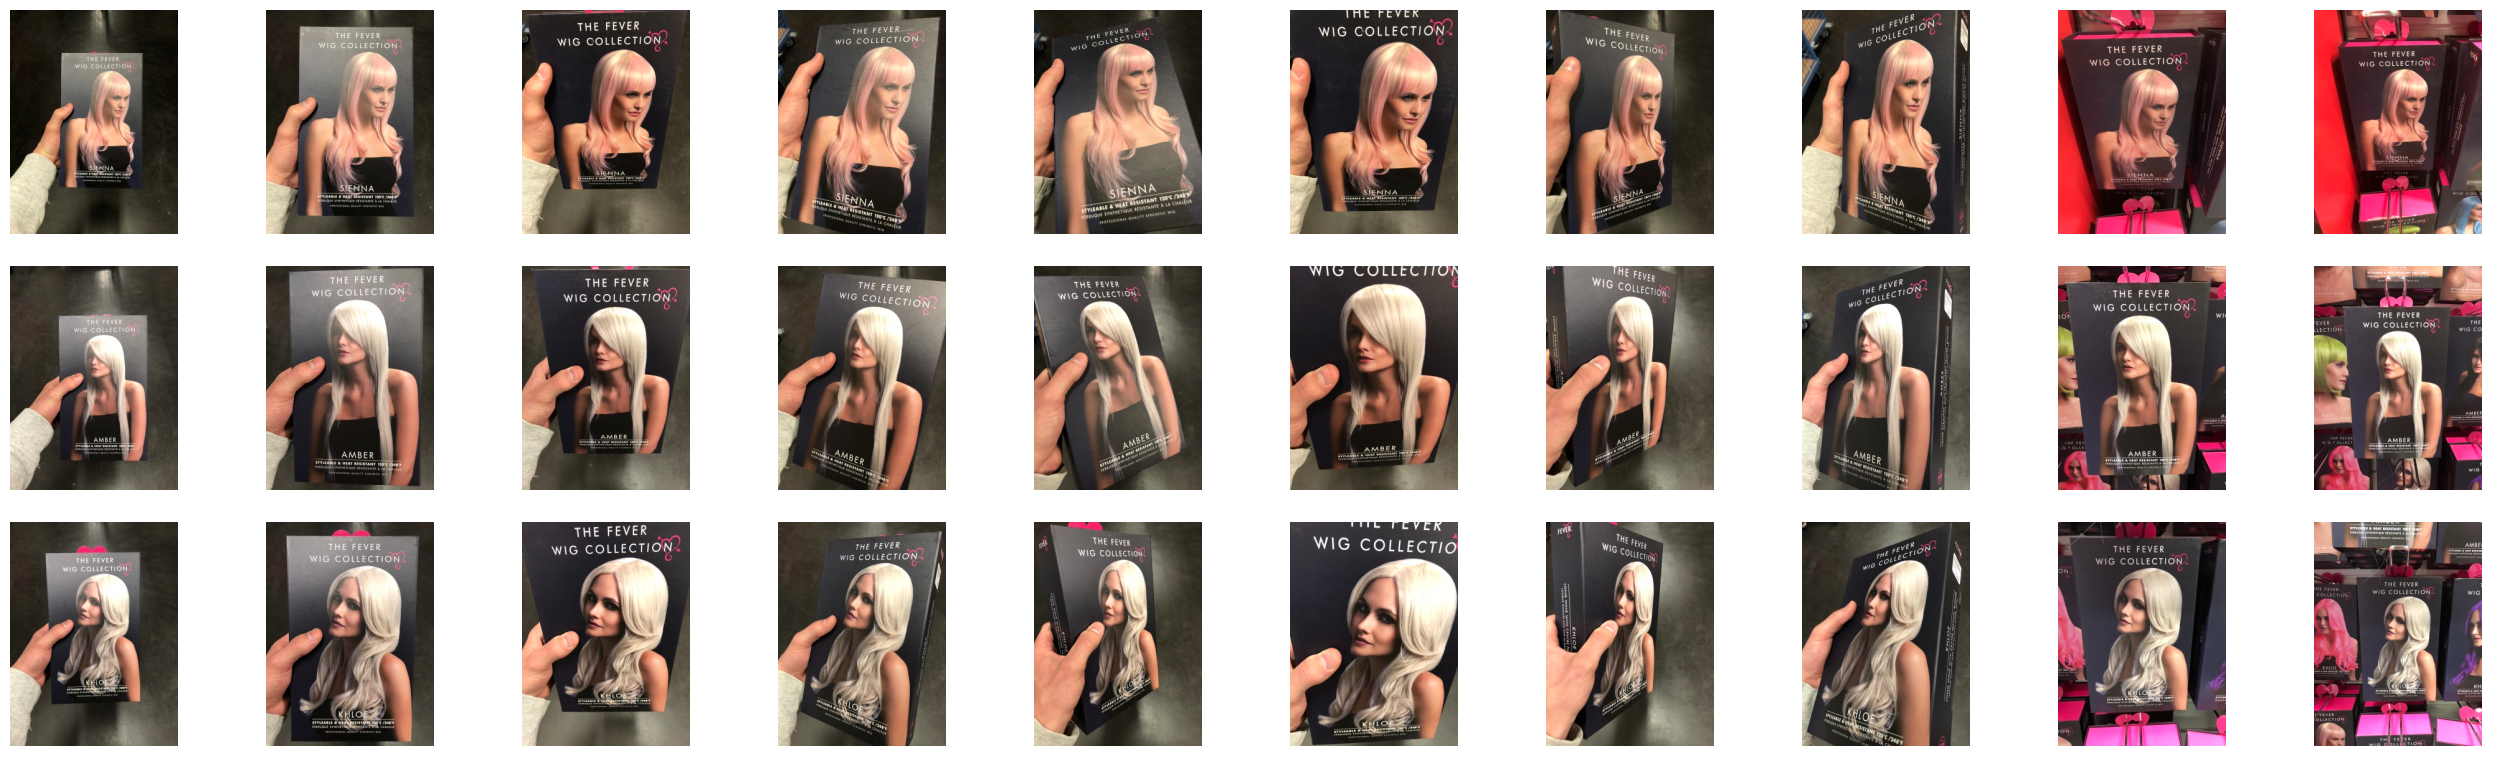
\includegraphics[width=1\textwidth]{img/testmiddel.png}
    \caption{Testdata voor middelgrote producten}
    \label{fig:testmiddel}
  \end{figure}

  \begin{figure}[h!]
    \centering
        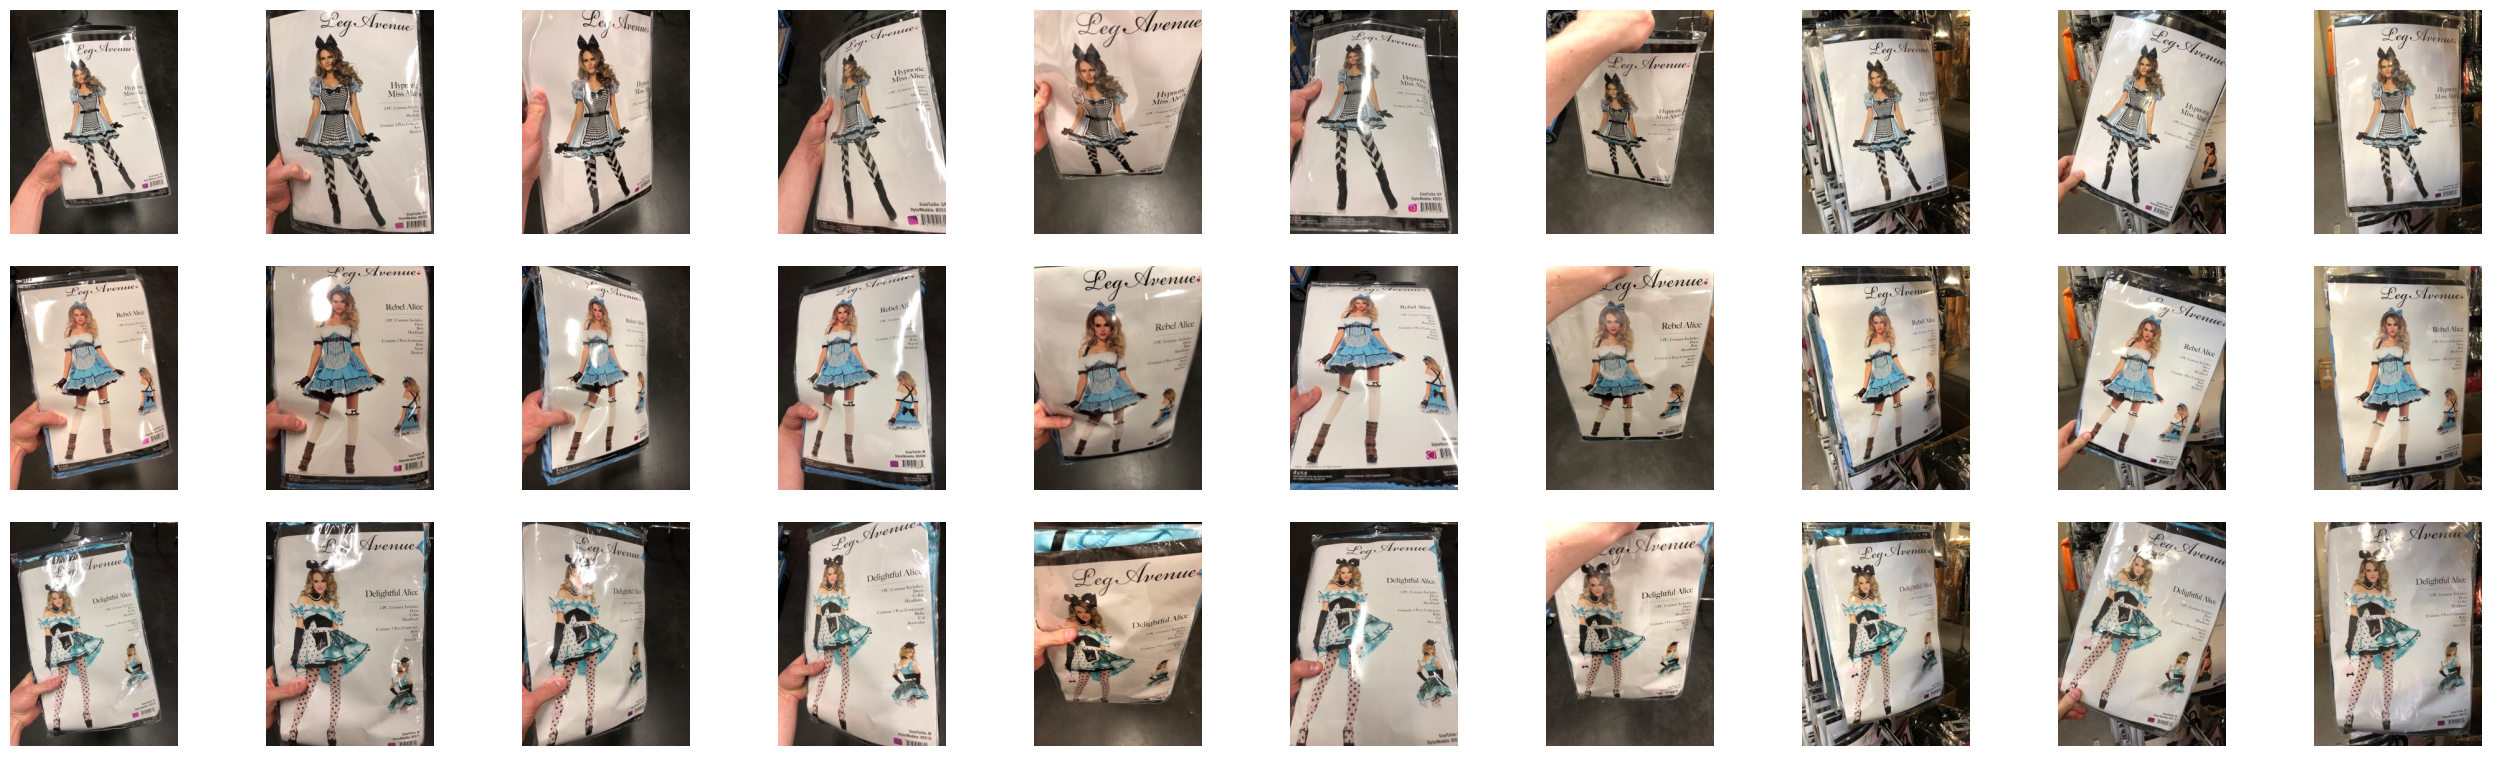
\includegraphics[width=1\textwidth]{img/testgroot.png}
    \caption{Testdata voor grote producten}
    \label{fig:testgroot}
  \end{figure}

\section{Testapplicatie}
\label{sec:Testapplicatie}

De testapplicatie heeft als doel vast te stellen hoeveel testafbeeldingen er juist worden herkend per framework. De testapplicatie is ontwikkeld met het programma Xcode, de gratis software voor Macgebruikers om iOS applicaties te programmeren. Er wordt eerst een testafbeelding ingeladen via de camera roll. Daarna wordt de afbeelding verkleind tot het gewenste inputformaat voor elk framework. Vervolgens wordt de waarschijnlijkheid dat de afbeelding tot een van de drie klasses behoord per framework getoond. Er zal dan gecontroleerd kunnen worden of de klasse met de hoogste waarschijnlijkheid ook effectief je juiste klasse is. De testapplicatie wordt voor zowel kleine, middelgrote als grote producten gebruikt steeds met bijhorend getrainde frameworks.  
  
\begin{figure}
    \centering
        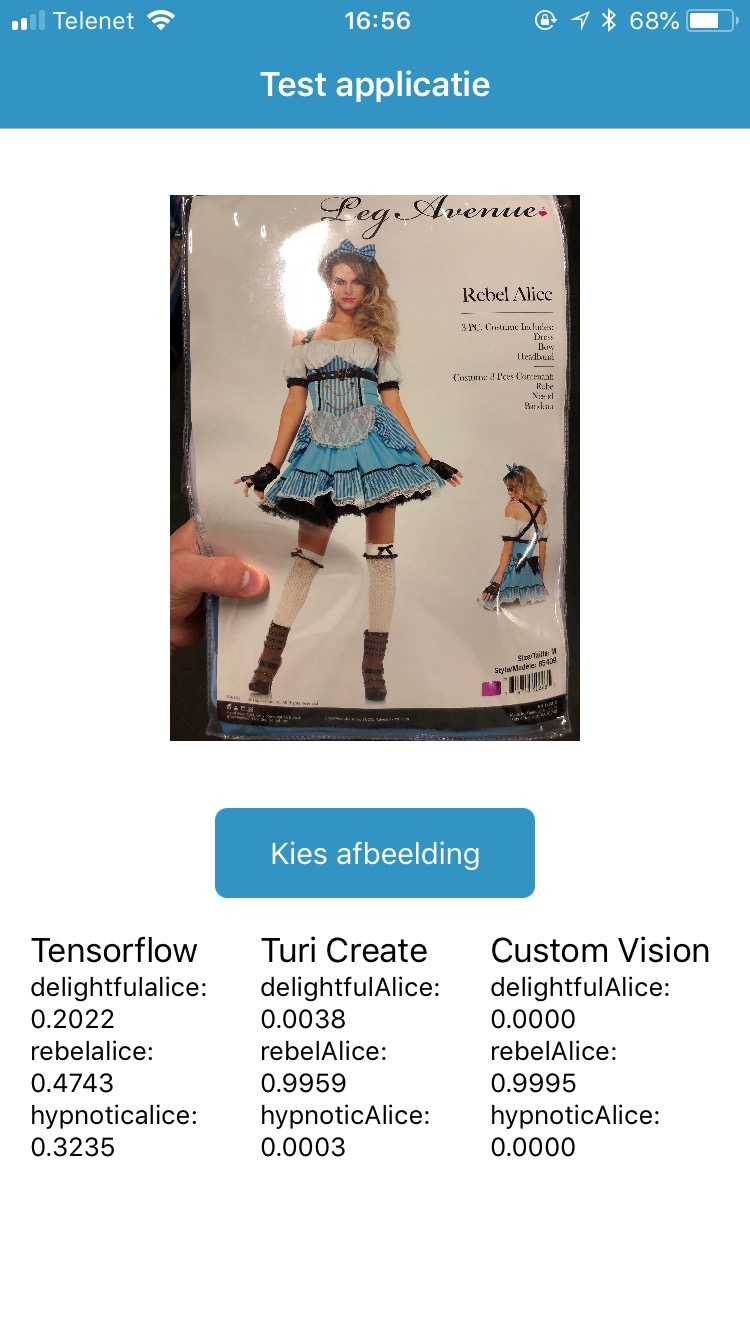
\includegraphics[width=0.3\textwidth]{img/testapplicatie.jpg}
    \caption{Voorbeeld van de testapplicatie}
    \label{fig:testapplicatie}
  \end{figure}
